% This text is proprietary.
% It's a part of presentation made by myself.
% It may not used commercial.
% The noncommercial use such as private and study is free
% Sep. 2005 
% Author: Sascha Frank 
% University Freiburg 
% www.informatik.uni-freiburg.de/~frank/


\documentclass[hyperref={pdfpagelabels=false}]{beamer}
\usepackage{graphicx,lmodern,subfigure,ulem,color,graphicx,tikz,booktabs,natbib}
\usepackage{mathrsfs}
\usetheme{default}
%\definecolor{beamer@blendedblue}{rgb}{0.1,0.5,0.1}
%\definecolor{ForestGreen}{RGB}{60, 140, 60}
%\setbeamercolor{structure}{fg=beamer@blendedblue}
\setbeamertemplate{navigation symbols}{}
\setbeamertemplate{footline}[frame number]
\bibliographystyle{chicago}
\newcommand{\ourname}{ProSocial}
\newcommand{\ourtoken}{Donum}

\setbeamersize{text margin left=2mm,text margin right=2mm} 

\title[Debt choice in a search model]{\ourname: A Decentralized Market for Public Goods} 
\author{\ourname}
\institute{Boston College}

\date{\today}

\begin{document}
	\frame{\titlepage \begin{center} Micro Theory Brown Bag, Boston College \end{center} }
	
	
	\frame{\frametitle{Why aren't we nicer to each other?}
		\begin{figure}
			\centering
			\begin{itemize}
				\item[] \textbf{What do you mean nice?} 
				\item Not this: I give you 5 dollars, you make me lunch.
				\item This: You do something expecting nothing in return.
				\item \textit{Non-Excludable Public Goods/Deeds}
				\begin{itemize}
					\item Writing a honest product review.
					\item Cleaning up a park.
					\item Moderating on-line forums.
					\item Volunteer work.
				\end{itemize}
				\vspace{0.1in}
				\item[] \textbf{Ever benefit from such public goods?} 
				\item Yes... 
				\vspace{0.1in}
				\item[] \textbf{Ever paid for this kind of work?} 
				\item Not so much...
			\end{itemize}
		\end{figure}
	}
	
		\frame{\frametitle{Where's the market?}
		\begin{figure}
			\centering
			\begin{itemize}
				\item[] \textbf{What do you pay?} 
				\item What's the right price? Depends on ``for what'' and ``to whom''.
				\item Must you pay? Most don't pay anyway... so why pay?
				\vspace{0.1in}
				\item[] \textbf{Payment issues} 
				\item Where do you put the money? 
				\item How do you send the money? To whom?
				\item Transaction costs and collection is a technological challenge.
				\vspace{0.1in}
				\item[] \textbf{Status Quo: ``Suboptimal'' production of public goods/deeds} 
				\item We produce fewer public goods that we would like to see produced.
				\item Only those who get the warm glow (meaning, they have a full stomach) from these goods produce them. 
			\end{itemize}
		\end{figure}
	}

	\frame{\frametitle{What are existing solutions?}
		\begin{figure}
			\centering
			\begin{itemize}
				\item[] \textbf{Charity} 
				\item Who donates? What are their motives?
				\item The wealthy decide which values are rewarded.
				\vspace{0.1in}
				\item[] \textbf{Taxes} 
				\item We vote for a government who levies taxes.
				\item Fundamentally good so long government remains ``good'' and ``'elected'. 
				\item Government cannot and should not provide many goods mentioned -- Honest product reviews, free financial advise, instructions on how to fix a car, or handle bankruptcy.
				\vspace{0.1in}
				\item[] \textbf{Praise} 
				\item ``We will miss a good man...''
				\item Upvote, like, retweet, thumbsup, share, forward. 
				\item We cannot survive on these societal affirmations.
			\end{itemize}
		\end{figure}
		\begin{center}
			{\color{red}\Large Can we incentivize public goods without imposing values?}
		\end{center}
	}

	\frame{\frametitle{This Presentation: Public goods in ONLINE communities}
		\begin{figure}
			\centering
			\begin{itemize}
				\item[] \textbf{Protocol} 
				\item From the real world to virtual communities
				\item A reward system with single dimension preferences
				\item Extending to more general preferences and scenarios
				\vspace{0.1in}
				\item[] \textbf{Implementation} 
				\item Sketch the final product
				\item Briefly outline challenges in implementation
				\begin{itemize}
					\item Proof-Of-Humanity to secure and extend the Blockchain
					\item Financing/Funding with Smart-Contracts
				\end{itemize}
				\vspace{0.1in}
				\item[] \textbf{Issues} 
				\item Outline different ways of gaming the system
				\item Unintended consequences
				\item Why does each feature exist?
			\end{itemize}
		\end{figure}
	}


	\begin{frame}
	\frametitle{Protocol: Public goods are non-excludable}
		\begin{figure}
		\centering
		
\includegraphics[scale=1.5]{110602-G-JG957-182_Low1}
		\caption{Who pays? Did everyone pay?}
		\label{fig:110602-G-JG957-182_Low1}
		\end{figure}
	\end{frame}
	
	\begin{frame}
	\frametitle{Protocol: Even if they are excludable... What is the price?}
		\begin{figure}
			\centering
			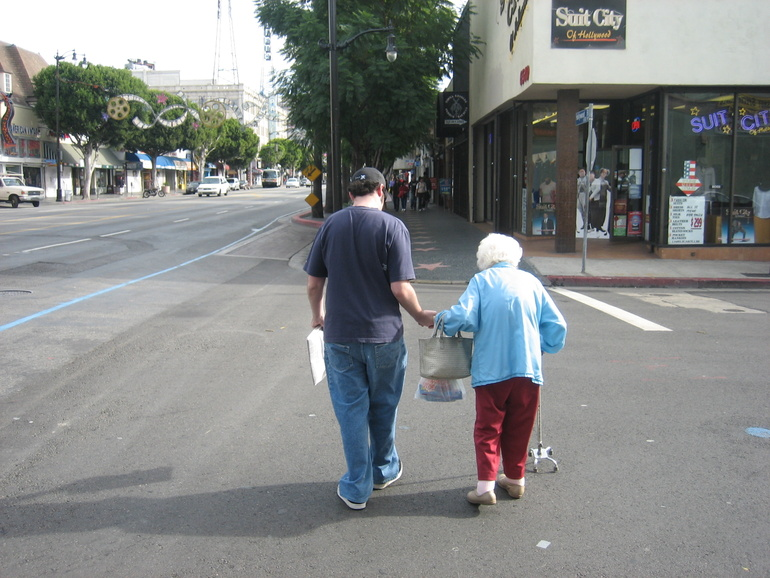
\includegraphics[scale=0.85]{Help-Old-Lady}
			\caption{How do you pay?}
			\label{fig:Help-Old-Lady}
		\end{figure}
	\end{frame}	
	
	\begin{frame}
	\frametitle{Protocol: One treasure, another's trash}
		\begin{figure}
			\centering
			
\includegraphics[scale=0.45]{sardine_icecream_en}
			\caption{Is it even a good? Who decides?}
			\label{fig:sardine_icecream_en}
		\end{figure}
	\end{frame}

	\frame{\frametitle{Protocol: From real world to virtual (sub)communities}
		\begin{figure}
			\centering
			
\includegraphics[scale=0.3]{the_donald}
			\caption{Virtual Communities \textbf{easily} form around \textbf{like-minded} people}
			\label{fig:the_donald}
		\end{figure}
	}

	\frame{\frametitle{Protocol: Virtual payments are substantially easier}
		\begin{figure}
			\centering
			
\includegraphics[scale=0.3]{twitterpuppies}
			\caption{\textbf{Easy} ``payments''/affirmations: Retweets, likes, upvotes, etc}
			\label{fig:twitterpuppies}
		\end{figure}
	}
	
	\frame{\frametitle{Protocol: Preferences in one dimension}
	\textbf{Setting}
	\begin{enumerate}
		\item A single virtual community with no disagreement over what is ``good''.
		\item ``Goods'' cost effort to create. 
		\item Affirmations are limited and/or costly to give.
		\item Affirmations cannot be consumed. 
		\item Minimum consumption threshold, heterogeneous draws of income.
	\end{enumerate}
	}

	\frame{\frametitle{Protocol: More puppies please!}
		\begin{figure}
			\centering
			
\includegraphics[scale=0.28]{awwwww}
			\caption{Only those with a camera and time can produce content}
			\label{fig:awwwww}
		\end{figure}
	\centering{\color{red}\Large Assumption: $\sum_i u'(cuteness,\cdot)>\text{Cost'(Puppy Pic)}$}
	}

	\frame{\frametitle{Protocol: Key problem and economic solution}
		\textbf{Optimal taxes}
		\begin{enumerate}
			\item A planner taxes everyone $ u'_i(cuteness,\cdot) $.
			\item Pays the creator of the puppy the cost. 
			\item Everyone is clearly indifferent. 
			\item The planner redistributes $\sum_i u'(cuteness,\cdot) - \text{Cost'(Puppy Pic)} > 0$.
		\end{enumerate}
	\vspace{0.2in}
	\underline{Good but less important detailed questions:} \\
	Who is the planner? What are marginal utilities and costs? Who pays the tax? Who participates? How do you implement? What if people can't pay?\vspace{0.2in}
	\Large{\color{red}\underline{Takeaway:} \\ An improvement is possible. How close can we get to it?}
	}
	
	\frame{\frametitle{Protocol: Implementation in One Community}
		\begin{enumerate}
			\item In each $ \Delta t $, a Bitcoin dividend (funded by a donor) is issued.
			\item The dividend is distributed proportionally to token holdings.
			\item Each user may give a token in each period $ \Delta t $.
			\item To give the token, the giver must keep his wallet active:
			\begin{itemize}
				\item prove humanity (captcha)
			\end{itemize}
			\item A token giver will also receive a token.
			\item All wallets depreciate at some natural rate $ \lambda_n $
			\item All wallets with updated proof-of-humanity depreciate at $ \lambda_h < \lambda_n$.
		\end{enumerate}
	}

	\frame{\frametitle{Protocol: Implementation with Multiple Communities}
		\begin{enumerate}
			\item In each $ \Delta t $, a Bitcoin dividend (funded by a donor for now) is issued
			\item The dividend is distributed proportionally to token holdings
			\item {\color{red}Each user may give $ w(j,t) $ tokens in each period $ \Delta t $ in any community.}
			\item {\color{red}$ w(j,t) $ is the social weight assigned to community $ j $ at time $ t $.}
			\item To give the token, the giver must keep his wallet active:
			\begin{itemize}
				\item prove humanity (captcha)
				\item {\color{red}rank communities (the system gives a user 2 communities, he picks one)}
				\item[] alternative:, ranking of community members in \textbf{other} communities
				\item {\color{red}the community ranking determines $ w(j,t) $}
			\end{itemize}
			\item {\color{red}A token giver will also receive w(j,t) token}
			\item All wallets depreciate at some natural rate $ \lambda_n $
			\item All wallets with updated proof-of-humanity depreciate at $ \lambda_h < \lambda_n$.
		\end{enumerate}
	}

	\frame{\frametitle{Protocol: Where does this lead to?}
		\textbf{Features:}
		\begin{enumerate}
			\item Our protocol can be embedded into existing on-line communities.
			\item Community members retain full control over their own communities.
			\item A rogue community will simply be down-ranked by others.
			\item New communities can form if necessary.
			\item The protocol does not dictate what is good. 
			\item A donor cannot dictate where his donation goes it. 
			\item Impossible to centralize the production of tokens. 
			\item Possible to punish by down-voting and rewarding individual history.
		\end{enumerate}
	}

	\frame{\frametitle{Implementation: Graphical UI}
	\begin{figure}
		\centering
		
\includegraphics[scale=0.5]{ButtonNew}
	\end{figure}
}

	\frame{\frametitle{Implementation: Graphical UI}
		\begin{figure}
			\centering
			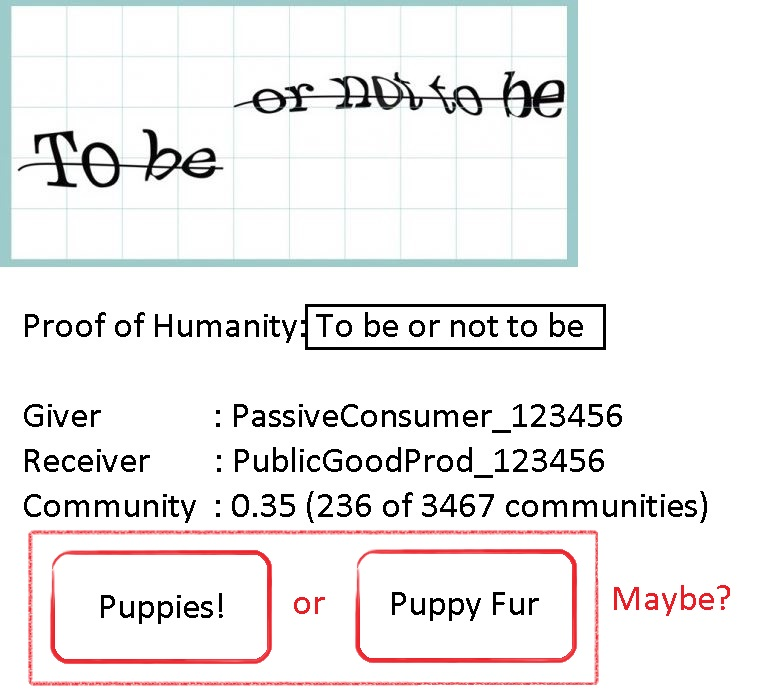
\includegraphics[scale=0.4]{PoH}
		\end{figure}
	}

	\frame{\frametitle{Implementation: Graphical UI}
	\begin{figure}
		\centering
		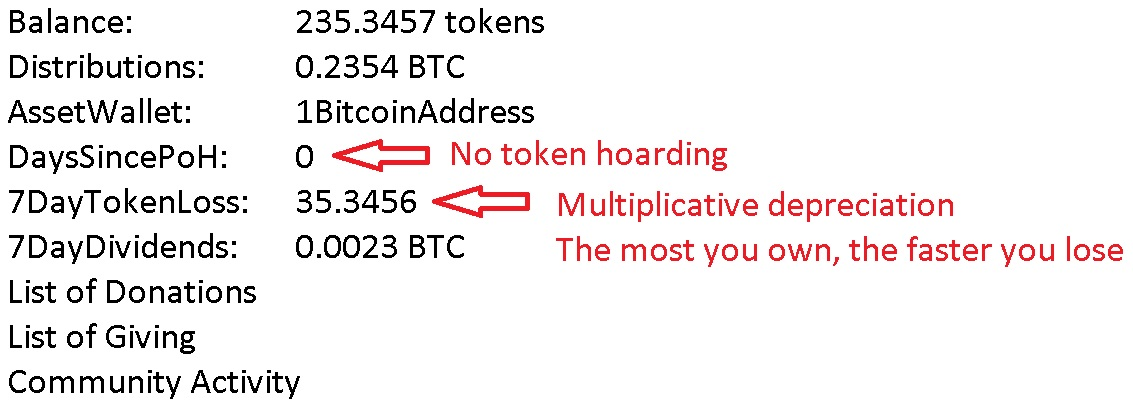
\includegraphics[scale=0.4]{WalletSnapShot}
	\end{figure}
	}
	

	\frame{\frametitle{Implementation: Proof-of-Humanity}
		\textbf{No know decentralized proof-of-humanity solution exists.}\\
		\vspace{0.2in}
		\textbf{Requirements}
		\begin{itemize}
			\item A human proves humanity by doing work costing \textbf{positive time}.
			\item The community can verify proof-of-humanity with much less work.
			\item Upgradeable to stay ahead of AI.
			\item Lightweight.
			\item \textbf{DECENTRALIZED}.
		\end{itemize}
	\vspace{0.1in}
	\begin{center}
		\Large{\color{red}Solution: Piggy back on existing projects. }
	\end{center}
	}

	\frame{\frametitle{Implementation: Funding}
		\textbf{Possibilities}
		\begin{itemize}
			\item \textbf{Donations:} Buying tokens and reinvesting returns is a donation.
			\item \textbf{Purchase human intel:} Captcha style source of revenue.
			\item \textbf{Survey:} Pay to post questions? How to prevent spam?
			\item \textbf{Participation:} Pay to bring this reward system into a community.
		\end{itemize}
		Each of these has issues... 
	}

	\frame{\frametitle{Implementation: Why each feature exists}
		\begin{itemize}
			\item \textbf{Proof of Humanity:} Social mining and preventing unequal token distribution.
			\item \textbf{Community ranking:} Letting society decide which communities it values.
			\item \textbf{Wallet Decay:} Prevent unequal token distribution. Enables donations.
			\item \textbf{Give to Get:} Promote participation and accumulation tokens at public good providers providers
		\end{itemize}
	}

	\frame{\frametitle{Conclusion}
		\begin{itemize}
			\item Sketched a system where public goods are encouraged without a donor dictating what goods should be created.
			\item Using Proof of Humanity mitigates inequality in the redistribution system.
			\item Resources accumulate to those who produce these public goods without the influence of a third party or a central organizer.
			\item How to bring money to the system remains a challenge. We assume donations for now.
		\end{itemize}
	}
\end{document}

